%
% codage CTE-OPEN
%
\subsubsection{Nouveau codage QBF par liens causaux: CTE-OPEN}

% %In SAT planning, each copy of the variable set $X$ is indexed, making the writing of transitions easy; let $P$ and $Q$ two formulas and $x_i$ and $x_{i+1}$ two copies of one variable

% Let $\F$ and $\A$ be two finite sets of \textit{fluents} and \textit{actions} respectively. With $\a \in \A$ an action, we define $\Cond{\a}$ as the set of fluents required to be true in the previous state for $\a$ to be executed and $\Add{\a}$ and $\Del{\a}$ the sets of added fluents (resp. removed) by the action $\a$. We also denote the set of all propositional variables by $\X$ where
% \[ \X = \A \cup \{\openSingle{f} ~|~ \f \in \F \}. \]

% We define a \textit{planning problem} as the tuple $\langle I, \A , G \rangle$ where $I \subseteq \F$ is the set of initial fluents, $G \subseteq \F$ is the set of goal fluents and $\A$ is the set of actions. A \textit{state} is an valuation of the set of fluents $\F$.

%{\color{blue} expliquer pourquoi on adapte le codage de MK99: pour ne pas avoir à dupliquer l'arbre QBF (on découpe les liens causaux en utilisant open)}

%\fred{Fred: La définition des $X_{i}$ et $b_{i}$ n'était donnée qu'après ce premier paragraphe (dans la partie \enquote{Quantifiers}). J'ai donc déplacé la définition du CTE dans la sous-section précédente en explicitant le cas des No-ops, et modifié les parties \enquote{Quantifiers} pour CTE-OPEN et CTE-EFA.}

Les codages SAT dans les espaces de plans de \cite{MK99} ne peuvent pas être directement adaptés au CTE. Tous ces codages se réfèrent à trois étapes indexées (pas nécessairement consécutives) du plan, ce qui n'est pas possible dans un CTE car chaque règle ne peut se référer qu'à des noeuds présents sur une même branche de l'arbre. Pour contourner ce problème, il serait possible de dupliquer l'arbre en ajoutant, pour chaque variable de branchement $b_{i}$, deux autres variables de branchement $b^{\prime}_{i}$ et $b^{\prime\prime}_{i}$, et pour chaque noeud $X_{i}$, deux copies de noeud $X^{\prime}_{i}$ et $X^{\prime\prime}_{i}$ , et les règles d'équivalence $\bigwedge_{x_{i}\in X_{i}} \big((x_{i}\leftrightarrow x^{\prime}_{i})\wedge (x_{i}\leftrightarrow x^{\prime\prime}_{i})\big)$. Malheureusement, cela augmenterait inutilement le facteur de branchement. Nous proposons donc un nouveau codage dans les espaces de plans qui nous permet de ne faire référence qu'à des étapes consécutives du plan.

Pour chaque variable $\f\in\F$, nous créons une variable propositionnelle $\openSingle{\f}$ pour exprimer que $\f$ se maintient à l'étape précédente et doit être protégé au moins jusqu'à l'étape en cours.
Dans la figure~\ref{fig:causal-link-cte}, la variable $f$ est une \textit {condition ouverte} à l'étape $\S_i$, impliquant que $\f\in\I$ ou une action $\b$ qui ajoute $\f$
est exécutée dans une étape précédente $\S_{i-j}$.
Les conditions ouvertes sont propagées vers l'arrière jusqu'à l'état initial ou jusqu'à une étape dans laquelle elles sont ajoutées par une action.


\begin{figure}[hb!]\centering
	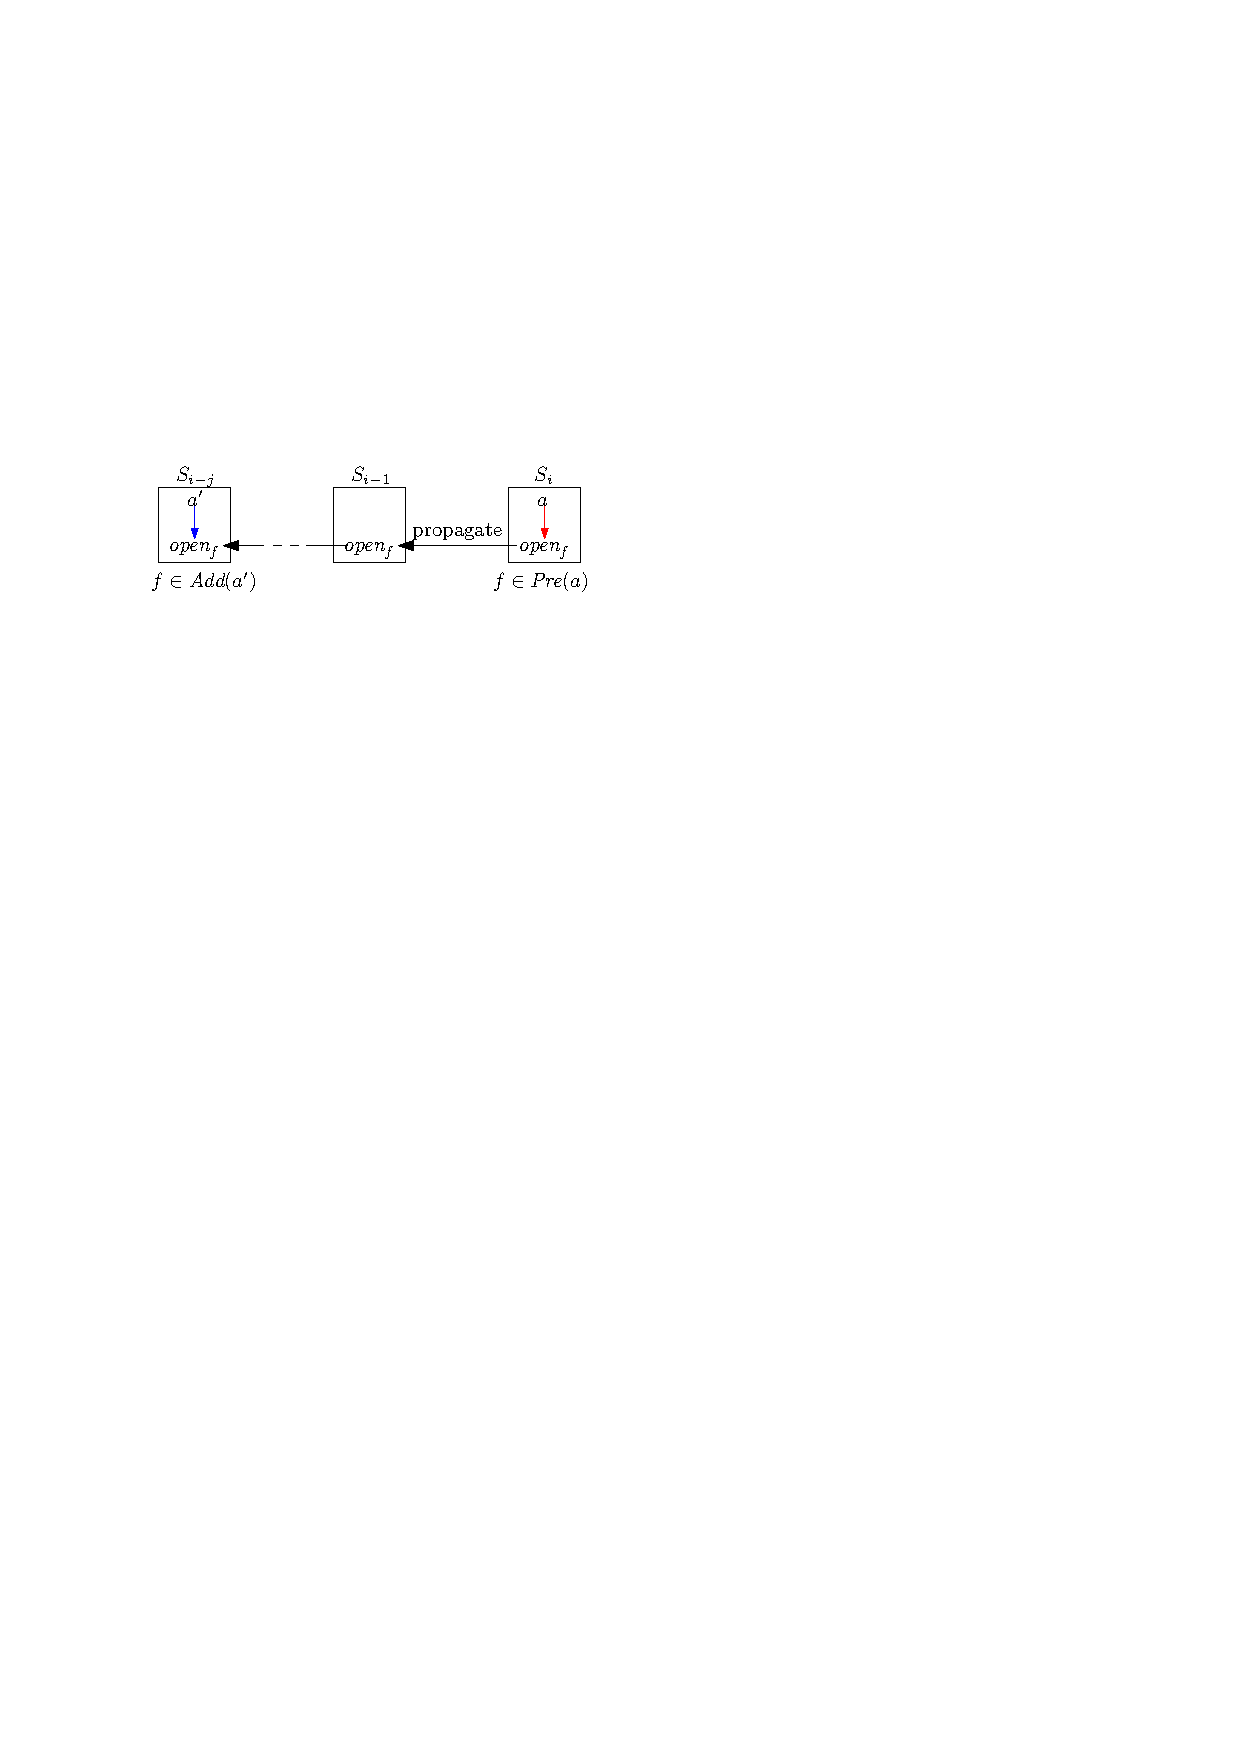
\includegraphics[width=.5\textwidth]{figures/transitions}
    \caption{Lien causal: $\b$ produit $\f$ pour $\a$.}
    \label{fig:causal-link-cte}
\end{figure}

Nous définissons l'ensemble des variables \enquote{open}, noté $\openSet$, comme $\openSet = \{\openSingle{\f} ~|~ \f \in \F \}$. Chaque action étant considérée comme une variable propositionnelle, nous définissons un ensemble de variables propositionnelles $\X$, donné par $\X = \A \cup \openSet$.


\paragraph*{[CTE-OPEN.0 -- Quantificateurs]}

Pour chaque profondeur $i$ de l'arbre, $\X_i$ dénote une copie de l'ensemble des variables $\X$ \fred{à reformuler}. Il existe une seule variable $\instepcte{\a}{i}\in X_{i}$ pour chaque action utilisée pour déterminer la dernière transition dans le plan et une seule variable $\openstepcte{\f}{i}\in X_{i}$ pour chaque fluent utilisée pour déterminer si $\f$ est une condition ouverte. A la même profondeur~$i$, la valeur de ces variables dépend du n\oe ud (correspondant à une étape du plan) sélectionné par les valeurs des variables universelles de branchement supérieures $b_{i+1}\ldots b_{\depth}$.

%\begin{small}
%\[
%\begin{matrix}
%\displaystyle \bigexists_{\a \in \A} \a_{\depth}. \bigexists_{\f\in \F} %\open{\f}{\depth}.%\\
%\displaystyle {\bigforall b_{\depth}.}\\
%\displaystyle \bigexists_{\a \in \A} \a_{\depth-1}. \bigexists_{\f\in \F} %\open{\f}{\depth-1}.%\\
%\displaystyle {\bigforall b_{\depth-1}.}\\
%\displaystyle \dots\\ 
%%\dots
%\displaystyle \bigexists_{\a \in \A} \a_{1}. \bigexists_{\f\in \F} %\open{\f}{1}.%\\
%\displaystyle {\bigforall b_{1}.}%\\
%\displaystyle \bigexists_{\a \in \A} \a_{0}. \bigexists_{\f\in \F} %\open{\f}{0}.
%\end{matrix}
%\]
%\end{small}\\

\begin{small}
\[
\begin{matrix}
\displaystyle \bigexists_{\a \in \A} \instepcte{\a}{\depth}. \bigexists_{\f\in \F} \openstepcte{\f}{\depth}.%\\
\displaystyle {\bigforall b_{\depth}.}\\
\displaystyle \bigexists_{\a \in \A} \instepcte{\a}{\depth-1}. \bigexists_{\f\in \F} \openstepcte{\f}{\depth-1}.%\\
\displaystyle {\bigforall b_{\depth-1}.}\\
\displaystyle \dots\\ 
%\dots
\displaystyle \bigexists_{\a \in \A} \instepcte{\a}{1}. \bigexists_{\f\in \F} \openstepcte{\f}{1}.%\\
\displaystyle {\bigforall b_{1}.}%\\
\displaystyle \bigexists_{\a \in \A} \instepcte{\a}{0}. \bigexists_{\f\in \F} \openstepcte{\f}{0}.
\end{matrix}
\]
\end{small}\\

%Dans ce qui suit, un \textit{n\oe ud} désigne maintenant un n\oe ud qui n'est pas une feuille. % et $\depth$ est la profondeur de l'arbre.
%Le prédécesseur d'un n\oe ud au niveau $i$ est la feuille la plus à droite du sous-arbre gauche. Le successeur d'un noeud au niveau $i$ est la feuille la plus à gauche du sous-arbre droit.
%Afin de sélectionner ces transitions, nous introduisons l'opérateur feuille-vers-n\oe ud $\leftselect{i}$ défini comme:
%%\begin{scriptsize}
%\[\leftselect{i} \equiv \neg b_{i} \wedge \BigforallTwo{j=1}{i-1} b_{j}.\]
%%\end{scriptsize}
%Symétriquement, nous introduisons l'opérateur n\oe ud-vers-feuille $\rightselect{i}$ défini comme:
%%\begin{scriptsize}
%\[\rightselect{i} \equiv b_{i} \wedge \BigforallTwo{j=1}{i-1} \neg b_{j}.\]
%%\end{scriptsize}

\paragraph*{[CTE-OPEN.1 -- Conditions ouvertes]}
%\displaystyle\mathop{\exists \a_{1}}_{\a \in \A} .\displaystyle\mathop{\exists \open{\f}{1}}_{\f\in \F} .\forall b_{1}. \displaystyle\mathop{\exists \a_{0}}_{\a \in \A} .\displaystyle\mathop{\exists \open{\f}{0}}_{\f\in \F} .\\
Si une action $\a$ est exécutée dans une étape du plan, alors chaque précondition de $\a$ doit être une condition ouverte à cette étape (c'est-à-dire qu'un lien causal est requis pour cette précondition).
%\begin{scriptsize}
%\[ \BigforallTwo{i=0}{\depth} \Bigforall{\a \in \A} \left(\a_{i} \Rightarrow \Bigforall{\f\in \Cond{\a}} \open{\f}{i}\right) \]
%\end{scriptsize}

\begin{small}
\[ \BigforallTwo{i=0}{\depth} \Bigforall{\a \in \A} \left(\instepcte{\a}{i} \Rightarrow \Bigforall{\f\in \Cond{\a}} \openstepcte{\f}{i}\right) \]
\end{small}

Dans la dernière étape du plan menant au but (c'est-à-dire la feuille la plus à droite de l'arbre), tous les fluents du but doivent être des conditions ouvertes ou ajoutées par des actions exécutées dans cette étape.
%\begin{scriptsize}
%\[ \BigforallTwo{i=1}{\depth}b_{i} \Rightarrow \Bigforall{\f\in G} \left(\open{\f}{0} \vee \bigvee\limits_{\substack{\a \in \A \\ \f \in \Add{\a}}} \a_{0}\right) \]
%\end{scriptsize}

\begin{small}
\[ \BigforallTwo{i=1}{\depth}\instepcte{b}{i} \Rightarrow \Bigforall{\f\in G} \left(\openstepcte{\f}{0} \vee \bigvee\limits_{\substack{\a \in \A \\ \f \in \Add{\a}}} \instepcte{\a}{0}\right) \]
\end{small}

\paragraph*{[CTE-OPEN.2 -- Propagation et fermeture]}

Aucune condition ne doit rester ouverte dans la première étape du plan (c'est-à-dire la feuille la plus à gauche de l'arbre) si elle n'est pas présente dans l'état initial.
%\begin{scriptsize}
%\[ \BigforallTwo{i=1}{\depth}\neg b_{i} \Rightarrow \Bigforall{\f\in \F\setminus I} \neg \open{\f}{0} \]	
%\end{scriptsize}

\begin{small}
\[ \BigforallTwo{i=1}{\depth}\neg \instepcte{b}{i} \Rightarrow \Bigforall{\f\in \F\setminus I} \neg \openstepcte{\f}{0} \]	
\end{small}

Toute condition ouverte dans une étape doit, soit rester ouverte, soit être ajoutée (fermée) par une action à l'étape précédente.

%\begin{scriptsize}
%\[ \BigforallTwo{i=1}{\depth} \Bigforall{\f\in \F} \left(\left(\open{\f}{i} \wedge \leftselect{i} \right) \Rightarrow \left(\open{\f}{0} \vee \bigvee\limits_{\substack{\a \in \A \\ \f \in \Add{\a}}} \a_{0}\right)\right) \]
%
%\[ \BigforallTwo{i=1}{\depth}\Bigforall{\f\in \F}\left(\left(\open{\f}{0} \wedge \rightselect{i} \right) \Rightarrow \left(\open{\f}{i} \vee \bigvee\limits_{\substack{\a \in \A \\ \f \in \Add{\a}}} \a_{i}\right)\right)
%\]
%\end{scriptsize}

\begin{small}
\[ \BigforallTwo{i=1}{\depth} \Bigforall{\f\in \F} \left(\left(\openstepcte{\f}{i} \wedge \leftselect{i} \right) \Rightarrow \left(\openstepcte{\f}{0} \vee \bigvee\limits_{\substack{\a \in \A \\ \f \in \Add{\a}}} \instepcte{\a}{0}\right)\right) \]

\[ \BigforallTwo{i=1}{\depth}\Bigforall{\f\in \F}\left(\left(\openstepcte{\f}{0} \wedge \rightselect{i} \right) \Rightarrow \left(\openstepcte{\f}{i} \vee \bigvee\limits_{\substack{\a \in \A \\ \f \in \Add{\a}}} \instepcte{\a}{i}\right)\right)
\]
\end{small}


 \paragraph*{[CTE-OPEN.3 -- Protection des conditions ouvertes]}

Une condition ouverte dans une étape donnée ne peut pas être supprimée à l'étape précédente. Cela garantit de ne rompre aucun lien de causalité dans le plan.
%\begin{scriptsize}
%\[ \BigforallTwo{i=1}{\depth} \Bigforall{\f\in \F}\left(\left(\open{\f}{i} \wedge \leftselect{i} \right) \Rightarrow \Bigforall{\a \in \A\\ \f \in \Del{\a}}\neg \a_{0}\right) \]
%\[ \BigforallTwo{i=1}{\depth} \Bigforall{\f \in \F} \left(\left(\open{\f}{0} \wedge \rightselect{i} \right) \Rightarrow \Bigforall{\a \in \A \\ \f \in \Del{\a}}\neg \a_{i}\right) \]
%\end{scriptsize}

\begin{small}
\[ \BigforallTwo{i=1}{\depth} \Bigforall{\f\in \F}\left(\left(\openstepcte{\f}{i} \wedge \leftselect{i} \right) \Rightarrow \Bigforall{\a \in \A\\ \f \in \Del{\a}}\neg \instepcte{\a}{0}\right) \]
\[ \BigforallTwo{i=1}{\depth} \Bigforall{\f \in \F} \left(\left(\openstepcte{\f}{0} \wedge \rightselect{i} \right) \Rightarrow \Bigforall{\a \in \A \\ \f \in \Del{\a}}\neg \instepcte{\a}{i}\right) \]
\end{small}

\paragraph*{[CTE-OPEN.4 -- Prévention des interactions négatives]}

Si une action supprime un fluent qui est nécessaire ou est ajouté par une autre action, alors ces deux actions ne peuvent pas être exécutées toutes les deux dans une même étape.
%\begin{scriptsize}
%\[ \BigforallTwo{i=0}{\depth} \Bigforall{\a \in \A} \Bigforall{\f\in \left(\Add{\a} \cup \Cond{\a}\right)} \Bigforall{\b \in \A \\ \a \neq \b \\ \f \in \Del{\b}}\left(\neg \a_{i} \vee \neg \b_{i}\right) \]
%\end{scriptsize}

\begin{small}
\[ \BigforallTwo{i=0}{\depth} \Bigforall{\a \in \A} \Bigforall{\f\in \left(\Add{\a} \cup \Cond{\a}\right)} \Bigforall{\b \in \A \\ \a \neq \b \\ \f \in \Del{\b}}\left(\neg \instepcte{\a}{i} \vee \neg \instepcte{\b}{i}\right) \]
\end{small}